\chapter{Probability}
\label{probability}

\index{probability|(} 

What are the chances that a woman with an abnormal mammogram has breast cancer?  What is the likelihood that an overweight male teenager with high blood pressure will develop cardiovascular disease by the age of 50?  What is the probability that two parents who are unaffected carriers of a genetic mutation that causes cystic fibrosis will have a child that suffers from the disease. All of these questions use the language of probability, and despite how easy it is to ask these questions,  answers are not always easy to come by.  Probability also forms the foundation for data analysis and statistical inference, since nearly every conclusion to a study should be accompanied by a measure of uncertainty.  In the publication of  LEAP study discussed in Chapter 1, the manuscript included the probability that the results of the study could have been due simply to chance variation (a very small probability, as will be seen later in the text).

Like all mathematical tools, probability becomes easier to understand and work with when the important concepts and language have been formalized.   With the right tools, seemingly difficult problems can be solved in a series of reliable, reproducible steps.  This chapter introduces that formalization, using two types of examples.  One set of examples uses familiar terms using settings most people have seen before -- the outcomes of rolling dice or picking cards from a deck of playing cards.  The second type of examples are drawn from medicine, biology or public health, and reflect the context and language used in those fields. The approaches to solving both types of problems are surprisingly similar, once the problem has been posed clearly.

\section{Defining probability}
\label{basicsOfProbability}

\subsection{Some examples}

\textit{Some of these dice examples can be dropped, but leaving them for now in case they are reference later. }

We begin with some familiar examples.

\begin{example}\label{dieAllOutcomesex}{A ``die'', the singular of dice, is a cube with six faces numbered \resp{1}, \resp{2}, \resp{3}, \resp{4}, \resp{5}, and \resp{6}. What is the chance of getting \resp{1} when rolling a die?}\label{probOf1}
If the die is fair, then the chance of a \resp{1} is as good as the chance of any other number. Since there are six outcomes, the chance must be 1-in-6 or, equivalently, $1/6$.
\end{example}

\begin{example}{What is the chance of getting a \resp{1} or \resp{2} in the next roll?}\label{probOf1Or2}
\resp{1} and \resp{2} constitute two of the six equally likely possible outcomes, so the chance of getting one of these two outcomes must be $2/6 = 1/3$.
\end{example}

\begin{example}{What is the chance of getting either \resp{1}, \resp{2}, \resp{3}, \resp{4}, \resp{5}, or \resp{6} on the next roll?}\label{probOf123456}
100\%. The outcome must be one of these numbers.
\end{example}

\begin{example}{What is the chance of not rolling a \resp{2}?}\label{probNot2}
Since the chance of rolling a \resp{2} is $1/6$ or $16.\bar{6}\%$, the chance of not rolling a \resp{2} must be $100\% - 16.\bar{6}\%=83.\bar{3}\%$ or $5/6$.

Alternatively, we could have noticed that not rolling a \resp{2} is the same as getting a \resp{1}, \resp{3}, \resp{4}, \resp{5}, or \resp{6}, which makes up five of the six equally likely outcomes and has probability $5/6$.
\end{example}

\begin{example}\label{dieProportionProbex} {Consider rolling two dice. If $1/6^{th}$ of the time the first die is a \resp{1} and $1/6^{th}$ of those times the second die is a \resp{1}, what is the chance of getting two \resp{1}s?}\label{probOf2Ones}
If $16.\bar{6}$\% of the time the first die is a \resp{1} and $1/6^{th}$ of \emph{those} times the second die is also a \resp{1}, then the chance that both dice are \resp{1} is $(1/6)\times (1/6)$ or $1/36$.
\end{example}

Here is an example from genetics.

\begin{example}
Cystic fibrosis (CF) is a life-threatening genetic disorder characterized by the buildup of thick mucus in the lungs and pancreas, caused by mutations in the \textit{CFTR} gene located on chromosome 7. Defective copies of \textit{CFTR} can result in the reduced quantity and/or function of the CFTR protein, which transports sodium and chloride across cell membranes. CF is an autosomal recessive disorder -- an individual only develops CF if they have inherited two affected copies of \textit{CFTR}. Individuals with one normal (wild-type) copy and one defective (mutated) copy are known as carriers; they do not develop CF, but may pass the disease-causing mutation onto their offspring.

Suppose that both members of a couple are CF carriers. What is the probability that a child of this couple will be affected by CF?  The problem sounds a bit more complicated than calculating probabilities for the outcome of rolling a die, but can be solved with the same simple methods.  We show two solutions.

\textit{Solution 1: Enumerate all of the possible outcomes and exploit the fact that the outcomes are equally likely, as in \ref{dieAllOutcomesex}  During reproduction, each parent passes along one copy of the \textit{CFTR} gene, with each copy passed along with probability 1/2. Figure \ref{fig:cfInheritance} shows the four possible genotypes for a child of these parents, with the paternal chromosome in blue, the maternal chromosome in green,  chromosomes with the wild-type and mutated version of CFTR marked with $+$ and$-$.  Each of the four outcomes (wild-type CFTR, wild-type CFTR),  (wild-type CFTR, CFTR mutation) (CFTR mutation, wild-type CFTR) and (CFTR mutation, CFTR mutation), so the child will be affected with probability $1/4$.  It is important to recognize that the child being an unaffected carrier consists of two distinct outcomes, not one.

\textit{Solution 2:  Calculate the proportion of outcomes that produce an affected child, as in \ref{dieProportionProbex}.}  During reproduction, half of the time, the mother will pass along an affected gene.  When the child receives an affected gene from the mother, about half of those times, the father will have passed along an affected gene.	So the proportion of times the child will be affected is $(1/2) \times (1/2) = 1/4$.
\end{example}

\begin{figure}
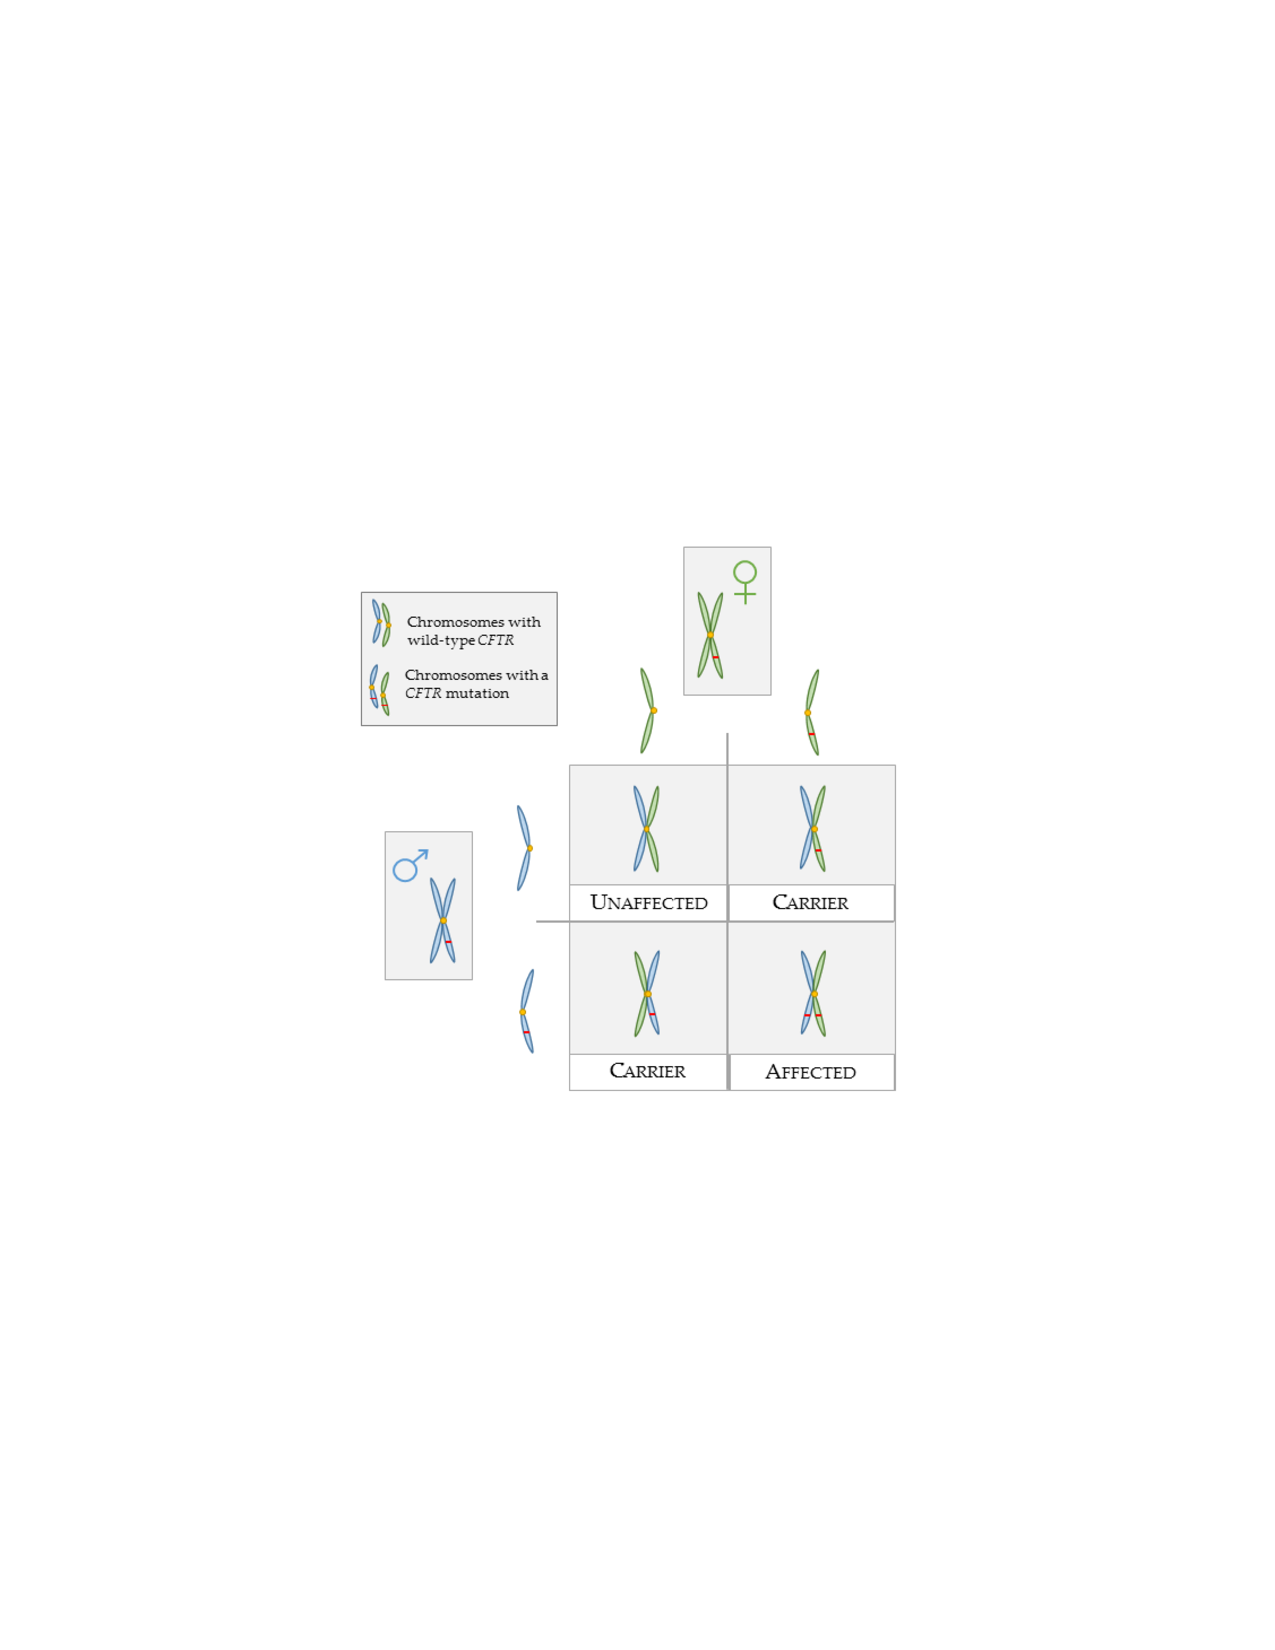
\includegraphics[width= 0.75\textwidth]{./figures/cfInheritance/cfInheritance.pdf}
\caption{Pattern of inheritance of a child of two unaffected carriers of CFTR}
\label{fig:cfInheritance}
\end{figure}


\begin{exercise}
Suppose the father is affected by CF and the mother is an unaffected carrier.  What is the probability that their child will be affected by the disease?

\textit{Solution}  Since the father is affected, he will always pass along a defective copy of the gene.  Since the mother will pass along a defective copy half of the time, the child will be affected half of the time, or with probability $1/4$.

\end{exercise}

\subsection{Probability}

\index{random phenomena |(}

Probability is used to assign a level of uncertainty to outcomes of phenomena that are happen randomly (rolling dice, passing along a defective gene during reproduction), or appear random because of a lack of understanding about exactly  how the phenomenon occurs (an obese teenager with high blood pressure developing cardiovascular disease later in life).In either case, the interpretation is the same -- the chance that some event will happen in the future -- and modeling these complex phenomena as random can be useful.

Mathematicians and philosophers have struggled for centuries (literally) to arrive at a clear statement of how probability is defined, or what it means.  In this text we use the most common definition, which also has the clearest interpretation.

\begin{termBox}{\tBoxTitle{Probability}
The \term{probability} of an outcome is the proportion of times the outcome would occur if the random phenomenon could be observed an infinite number of times.}
\end{termBox}

Probability is defined as a proportion, and it always takes values between 0~and~1 (inclusively). It may also be displayed as a percentage between 0\% and 100\%.

It is easy to imagine rolling dice a large number of times to observe the law of large numbers, but for examples like the CF example, the interpretation of probability is more hypothetical, since family sizes are typically small.  But it is not too difficult to imagine a thought experiment in which two parents have many children.  If the two parents are unaffected carriers, approximately 25\% of their off spring will suffer from CF.

This definition of probability can be illustrated by rolling a die many times. Let $\hat{p}_n$ be the proportion of outcomes that are \resp{1} after the first $n$ rolls. As the number of rolls increases, $\hat{p}_n$ will converge to the probability of rolling a \resp{1}, $p = 1/6$. Figure~\ref{dieProp} shows this convergence for 100,000 die rolls. The tendency of $\hat{p}_n$ to stabilize around $p$ is described by the \term{Law of Large Numbers}. 

\begin{figure}[bt]
\centering
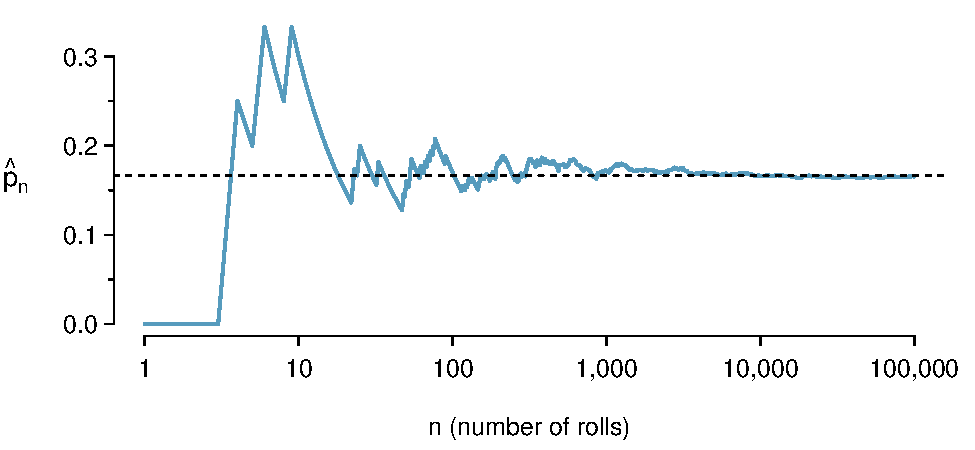
\includegraphics[width=0.85\textwidth]{ch_probability_oi_biostat/figures/dieProp/dieProp}
\caption{The fraction of die rolls that are 1 at each stage in a simulation. The proportion tends to get closer to the probability $1/6 \approx 0.167$ as the number of rolls increases.}
\label{fig:dieProp}
\end{figure}

The behavior shown in \ref{fig:dieProp} matches most people's intuition about probability, but proving mathematically that the behavior is always true is surprisingly difficult and is beyond the level of this text.  Mathematicians call the result \textit{The Law of Large Numbers}, which is used to justify mathematically this intuitively appealing definition.

\index{Law of Large Numbers |(}

\begin{termBox}{\tBoxTitle{Law of Large Numbers}
As more observations are collected, the proportion $\hat{p}_n$ of occurrences with a particular outcome converges to the probability $p$ of that outcome.}
\end{termBox}

Occasionally the proportion will veer off from the probability and appear to defy the Law of Large Numbers, as $\hat{p}_n$ does many times in Figure~\ref{dieProp}. However, these deviations become smaller as the number of rolls increases.

The notation $p$ is the probability of rolling a \resp{1}. We can also write this probability as
\begin{eqnarray*}
P(\text{rolling a \resp{1}})
\end{eqnarray*}
\marginpar[\raggedright\vspace{-13mm}

$P(A)$\vspace{1mm}\\\footnotesize Probability of\\outcome $A$]{\raggedright\vspace{-13mm}

$P(A)$\vspace{1mm}\\\footnotesize Probability of\\outcome $A$}As we become more comfortable with this notation, we will abbreviate it further. For instance, if it is clear that the process is ``rolling a die'', we could abbreviate $P($rolling a \resp{1}$)$ as~$P($\resp{1}$)$. 

\subsection{Disjoint or mutually exclusive outcomes}

\index{disjoint|(}
\index{mutually exclusive|(}

Two outcomes are called \term{disjoint} or \term{mutually exclusive} if they cannot both happen. For instance, if we roll a die, the outcomes \resp{1} and \resp{2} are disjoint since they cannot both occur. On the other hand, the outcomes \resp{1} and ``rolling an odd number'' are not disjoint since both occur if the outcome of the roll is a \resp{1}. The terms \emph{disjoint} and \emph{mutually exclusive} are equivalent and interchangeable.

Calculating the probability of disjoint outcomes is easy. When rolling a die, the outcomes \resp{1} and \resp{2} are disjoint, and we compute the probability that one of these outcomes will occur by adding their separate probabilities:
\begin{eqnarray*}
P(\text{\resp{1} or \resp{2}}) = P(\text{\resp{1}})+P(\text{\resp{2}}) = 1/6 + 1/6 = 1/3
\end{eqnarray*}
What about  the probability of rolling a \resp{1}, \resp{2}, \resp{3}, \resp{4}, \resp{5}, or \resp{6}? Here again, all of the outcomes are disjoint so we add the probabilities:
\begin{eqnarray*}
&&P(\text{\resp{1} or \resp{2} or \resp{3} or \resp{4} or \resp{5} or \resp{6}}) \\
	&&\quad= P(\text{\resp{1}})+P(\text{\resp{2}})+P(\text{\resp{3}})+P(\text{\resp{4}})+P(\text{\resp{5}})+P(\text{\resp{6}}) \\
	&&\quad= 1/6 + 1/6 + 1/6 + 1/6 + 1/6 + 1/6 = 1.
\end{eqnarray*}
The \term{Addition Rule} guarantees the accuracy of this approach when the outcomes are disjoint. 

\begin{termBox}{\tBoxTitle{Addition Rule of disjoint outcomes} If $A_1$ and $A_2$ represent two disjoint outcomes, then the probability that one of them occurs is given by
\begin{eqnarray*}
P(A_1\text{ or } A_2) = P(A_1) + P(A_2)
\end{eqnarray*}
If there are many disjoint outcomes $A_1$, ..., $A_k$, then the probability that one of these outcomes will occur is
\begin{eqnarray}
P(A_1) + P(A_2) + \cdots + P(A_k)
\end{eqnarray}
}
\end{termBox}

\begin{exercise}
We are interested in the probability of rolling a \resp{1}, \resp{4}, or \resp{5}. (a) Explain why the outcomes \resp{1}, \resp{4}, and \resp{5} are disjoint. (b) Apply the Addition Rule for disjoint outcomes to determine $P($\resp{1} or \resp{4} or \resp{5}$)$.\footnote{(a) The random process is a die roll, and at most one of these outcomes can come up. This means they are disjoint outcomes. (b)~$P($\resp{1} or \resp{4} or \resp{5}$) = P($\resp{1}$)+P($\resp{4}$)+P($\resp{5}$) = \frac{1}{6} + \frac{1}{6} + \frac{1}{6} = \frac{3}{6} = \frac{1}{2}$}
\end{exercise}


